% Given a history, how each d_ik is computed: replay tau -> the fatal act -> each feature is a
% PIECEWISE rule of that act; from witness i's viewpoint the highlighted branch fires -> average x100 = U_i.
% Example: the samurai's suicide, scored for the bandit (his best feasible account, 58 in Fig 1c).
\documentclass[tikz,border=3pt]{standalone}
\usepackage{amsmath}
\usepackage{xcolor}
\usetikzlibrary{arrows.meta,calc,positioning}
\definecolor{db}{HTML}{2E5A9C}
\definecolor{sel}{HTML}{2E8B3D}
\newcommand{\hit}[1]{{\color{sel}\mathbf{#1}}}
\begin{document}
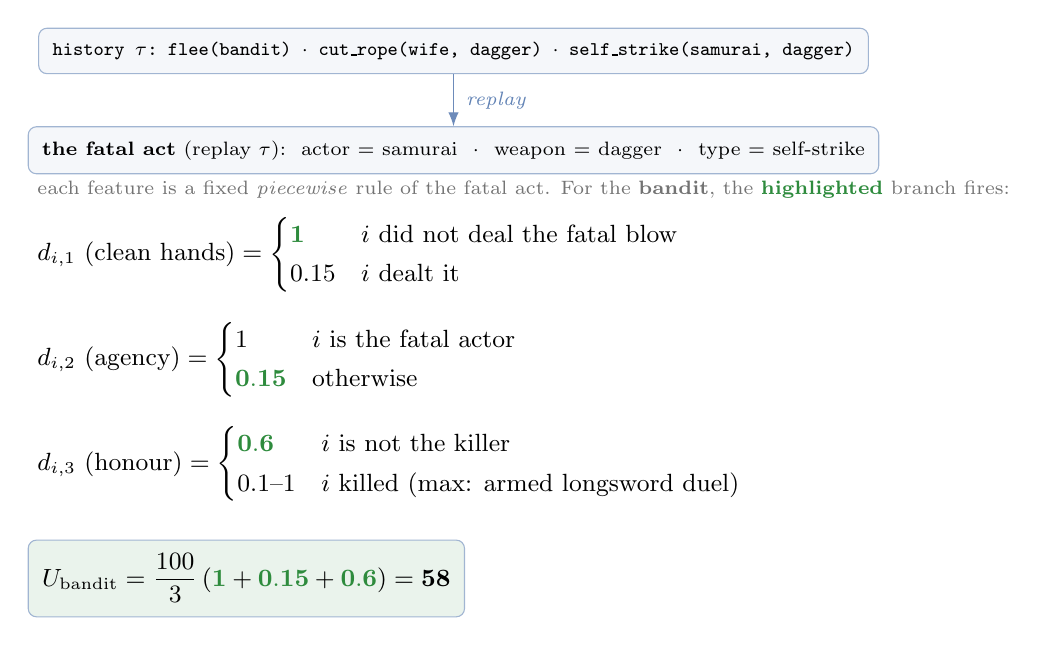
\begin{tikzpicture}[font=\sffamily, >={Latex[length=5pt]},
   stg/.style={draw=db!45, rounded corners=3pt, fill=db!5, inner sep=5pt, align=center}]
  \node[stg, font=\scriptsize\ttfamily] (h)
    {history $\tau$:\ flee(bandit) $\cdot$ cut\_rope(wife, dagger) $\cdot$ self\_strike(samurai, dagger)};
  \node[stg, below=0.66cm of h, font=\scriptsize] (s)
    {\textbf{the fatal act} (replay $\tau$):\ \ actor $=$ samurai\ \ $\cdot$\ \ weapon $=$ dagger\ \ $\cdot$\ \ type $=$ self-strike};
  \draw[->,db!70] (h)--(s) node[midway,right=1pt,font=\scriptsize\itshape,text=db!75]{replay};
  \node[below=0.5cm of s.west, anchor=west, font=\scriptsize, text=black!55, align=left] (lab)
    {each feature is a fixed \emph{piecewise} rule of the fatal act. For the \textbf{bandit}, the \textcolor{sel}{\textbf{highlighted}} branch fires:};
  \node[below=0.22cm of lab.west, anchor=north west, font=\small] (c1)
    {$d_{i,1}\ (\text{clean hands})=\begin{cases}\hit{1} & i \text{ did not deal the fatal blow}\\[1pt] 0.15 & i \text{ dealt it}\end{cases}$};
  \node[below=0.12cm of c1.south west, anchor=north west, font=\small] (c2)
    {$d_{i,2}\ (\text{agency})=\begin{cases} 1 & i \text{ is the fatal actor}\\[1pt] \hit{0.15} & \text{otherwise}\end{cases}$};
  \node[below=0.12cm of c2.south west, anchor=north west, font=\small] (c3)
    {$d_{i,3}\ (\text{honour})=\begin{cases} \hit{0.6} & i \text{ is not the killer}\\[1pt] 0.1\text{--}1 & i \text{ killed (max: armed longsword duel)}\end{cases}$};
  \node[stg, fill=sel!10, font=\small, below=0.35cm of c3.south west, anchor=north west] (u)
    {$U_{\text{bandit}}=\dfrac{100}{3}\,(\hit{1}+\hit{0.15}+\hit{0.6})=\mathbf{58}$};
\end{tikzpicture}
\end{document}
